
\marginnote[-2mm]{Ce théorème a été démontré par le mathématicien italien Guido \textsc{Fubini} en 1907.}
\begin{theo}{}
    Soit $f: [a,b] \times [c, d] \to \K$ une application continue. Alors,
    $$\int_{a}^{b} \left ( \int_{c}^{d} f(x,y) \d y \right) \d x = \int_{c}^{d} \left ( \int_{a}^{b} f(x,y) \d x \right) \d y.$$
\end{theo}

\begin{marginfigure}[5cm]
    \centering
    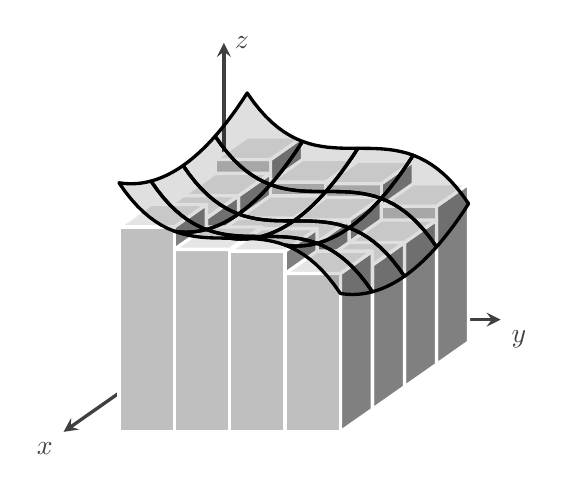
\begin{tikzpicture}[
  x=(215:2em/sqrt 2), y=(0:2em), z=(90:2em),
  declare function={f(\x,\y)=((\x-3)^2+(-\y+3)^3)/8+3;}, 
  very thick, line join=round]
\draw [-stealth, black!75] (0,0,0) -- (5,0,0) node [below left] {$x$};
\draw [-stealth, black!75] (0,0,0) -- (0,5,0) node [below right] {$y$};
\draw [-stealth, black!75] (0,0,0) -- (0,0,5) node [right] {$z$};
\foreach \x in {1,...,4}
  \foreach \y [evaluate={\j=\x+.5; \i=\y+.5; \k=f(\j,\i);}] in {1,...,4}{
    \path [fill=black!50, draw=white] (\x, \y+1, 0) -- (\x+1, \y+1, 0) -- 
      (\x+1, \y+1, \k) -- (\x, \y+1, \k) -- cycle;
    \path [fill=black!25, draw=white] (\x+1, \y, 0) -- (\x+1, \y+1, 0) -- 
      (\x+1, \y+1, \k) -- (\x+1, \y, \k) -- cycle;
    \path [fill=black!10, draw=white] (\x, \y, \k)  -- (\x+1, \y, \k) -- 
      (\x+1, \y+1, \k) -- (\x, \y+1, \k) -- cycle;
  }
 \foreach \x in {1,...,4}
   \foreach \y in {1,...,4}{
 \draw [black, fill=black, fill opacity=0.125, 
    domain=0:1, samples=10, variable=\t] 
    plot (\x+\t, \y, {f(\x+\t,\y)}) -- 
    plot (\x+1, \y+\t, {f(\x+1,\y+\t)}) -- 
    plot (\x+1-\t, \y+1, {f(\x+1-\t,\y+1)}) --
    plot (\x, \y+1-\t, {f(\x,\y+1-\t)}) -- cycle;
  }
\end{tikzpicture}
    \caption*{\centering Cette figure ne correspond pas au théorème de \textsc{Fubini}}
\end{marginfigure}

\textit{Correction du sujet Mines Maths 2 PSI 2021 par Doc Solus.} 
\begin{preuve}
    Pour tout $(x, t) \in [a, b] \times [c, d]$ on pose $\boxed{\varphi(x, t) \defeq \int_{a}^{x} f(u, t) \d u}$. 
    \begin{enumerate}
        \item Montrer que pour tout $x \in [a, b]$, l'application $t \mapsto \varphi(x, t)$ est continue sur $[c, d]$. \\
        Application du \textbf{théorème de continuité des intégrales à paramètre}. \\
        Pour la domination : $f$ est continue sur une partie fermée bornée de $\R^2$, donc d'après le \textbf{théorème des bornes}, $f$ est bornée sur $[a, b] \times [c, d]$ par une constante $M \in \Rp$.
        \item On pose alors, pour tout $x  \in [a, b],\ \boxed{\psi(x) \defeq \int_{c}^{d} \varphi(x, t) \d t}$. Montrer que $\psi$ est de classe $\mathscr{C}^1$ sur $[a, b]$, préciser $\psi'$. \\
        Application du \textbf{théorème de dérivation des intégrales à paramètre} à la fonction $x \mapsto \int_{c}^{d} \varphi(x, t) \d t$:
        \begin{itemize}
            \item $\forall t \in [c, d],\ x \mapsto \varphi(x, t)$ est de classe $\mathscr{C}^1$ sur $[a, b]$ car c'est la \textbf{primitive} s'annulant en $a$ de la fonction continue $x \mapsto f(x, t)$. 
            \item $\frac{\partial \varphi}{\partial x}(x, t) = f(x, t)$
            \item La domination se fait par le même constante $M$ que précédemment. 
        \end{itemize}
        $$\forall x \in [a, b] \quad \psi'(x) = \int_{c}^{d} f(x, t) \d t.$$
        \item En déduire:
        $$\forall x \in [a, b],\ \int_{a}^{x} \left ( \int_{c}^{d} f(u,t) \d t \right) \d u = \int_{c}^{d} \left ( \int_{a}^{x} f(u,t) \d u \right) \d t.$$
        Soit $x \in [a, b]$. D'une part,
        $$\psi(x) = \int_{c}^{d} \left ( \int_{a}^{x} f(u,t) \d u \right) \d t.$$
        D'autre part, d'après la question précédente et le \textbf{théorème fondamental de l'analyse}, 
        \begin{align*}
            \int_{a}^{x} \left ( \int_{c}^{d} f(u,t) \d t \right) \d u &= \int_{a}^{x} \psi'(u) \d u  = \psi(x) - \psi(a) \\
            \text{Or } \psi(a) &= \int_{c}^{d} \varphi(a, t)\ \d t \\
            \text{et } \forall t \in [c, d] \quad \varphi(a, t) &= \int_{a}^{a} f(u, t) \d u = 0
        \end{align*}
        d'où $\psi(a) = 0$ et le résultat. \\
        En particulier, pour $x = b$ on obtient le résultat final.
    \end{enumerate}
\end{preuve}    
